\documentclass[ucs, notheorems, handout, 10pt]{beamer}

\usetheme[numbers,totalnumbers,compress, nologo]{Statmod}
%\usetheme{Madrid}
\usefonttheme[onlymath]{serif}
\setbeamertemplate{navigation symbols}{}

\mode<handout> {
	\usepackage{pgfpages}
	\setbeameroption{show notes}
	\pgfpagesuselayout{2 on 1}[a4paper, border shrink=5mm]
	\setbeamercolor{note page}{bg=white}
	\setbeamercolor{note title}{bg=gray!10}
	\setbeamercolor{note date}{fg=gray!10}
}

\usepackage[utf8x]{inputenc}
\usepackage[T2A]{fontenc}
\usepackage[russian]{babel}
\usepackage{tikz}
\usepackage{ragged2e}
\usepackage{amsmath,amssymb,amsthm,amscd,amsfonts, mathabx}
\setbeamertemplate{caption}[numbered]

\newtheorem{theorem}{Теорема}
\newtheorem{defenition}{Определение}

\title[Оценивание значимости выравнивания]{Задачи оценивания значимости выравнивания при помощи скрытых марковских моделей}

\author[Власенко Д.В.]{Власенко Даниил Владимирович, гр.19.Б04-мм}

\institute[Санкт-Петербургский Государственный Университет]{%
	\small
	Научный руководитель: к.ф.-м.н. Коробейников А.И.\\ \vspace{0.5cm}
	Санкт-Петербургский государственный университет\\
	Прикладная математика и информатика\\
	Вычислительная стохастика и статистические модели\\
	\vspace{1.25cm}
	Отчет по производственной практике}

\date[Зачет]{Санкт-Петербург, 2022}

\subject{Talks}


\begin{document}
	
	\begin{frame}[plain]
		\titlepage
		
		\note{Научный руководитель  к.ф.-м.н., Коробейников А.И.,\\
			кафедра статистического моделирования}
	\end{frame}
	
	\begin{frame}{Введение}
		Пусть дан алфавит символов $\Sigma$. 
		\begin{defenition}Последовательностью длины $L$ над алфавитом $\Sigma$ будем называть такой $X$, что $X \in \Sigma^{L}$. Последовательностью $X$ над алфавитом $\Sigma$ будем называть такой $X$, что $X \in \bigcup_{L=0}^{L=\infty}\Sigma^{L}$.
		\end{defenition}
		
		Сходство последовательностей может отражать взаимосвязи объектов, которые они описывают. Например, такие как:

		\begin{center}
			\begin{itemize}
				\item функциональные,
				\item структурные,
				\item эволюционные.
			\end{itemize}
		\end{center}		 
		
		\note{
			Пусть дан алфавит символов $\Sigma$. 
			\begin{defenition}Последовательностью длины $L$ над алфавитом $\Sigma$ будем называть такой $X$, что $X \in \Sigma^{L}$. Последовательностью $X$ над алфавитом $\Sigma$ будем называть такой $X$, что $X \in \bigcup_{L=0}^{L=\infty}\Sigma^{L}$.
			\end{defenition}
			
			Сходство последовательностей может отражать функциональные, структурные или эволюционные взаимосвязи объектов, которые описывают эти последовательности. Таким образом умение находить взаимосвязи в строках может быть приложимо в задаче определения степени родства биологических организмов путем сравнения их ДНК или РНК, нуклеотидных последовательностей, задаче анализа свойств белков, аминокислотных последовательностей, задаче распознавания речи человека или письменного языка и многих других приложениях. 
		}
	\end{frame}

	\setcounter{framenumber}{1}
	\begin{frame}{Введение}
		\begin{defenition}
			Выравниванием $N$ последовательностей называется отображение $Q: \bigtimes_{i=1}^{N}(\bigcup_{L_i=0}^{\infty} \Sigma^{L_i}) \rightarrow \bigtimes_{i=1}^{N}(\Sigma^{L})$, где $L = \max(\{L_i\}_{i=1}^{N})$ такое что:
			\begin{enumerate}
				\item Возможны вставки символа --- в последовательностях.
				\item Вставка --- на одинаковых позициях во всех последовательностях запрещена.
				\item Порядок изначальных символов внутри последовательностей сохраняется.
			\end{enumerate}
		\end{defenition}
		
		Элементы из области значения $Q$ также называются выравниваниями.
		
		\note{
			\begin{defenition}
				Выравниванием $N$ последовательностей называется отображение $Q: \bigtimes_{i=1}^{N}(\bigcup_{L_i=0}^{\infty} \Sigma^{L_i}) \rightarrow \bigtimes_{i=1}^{N}(\Sigma^{L})$, где $L = \max(\{L_i\}_{i=1}^{N})$ такое что:
				\begin{enumerate}
					\item Возможны вставки символа --- в последовательностях.
					\item Вставка --- на одинаковых позициях во всех последовательностях запрещена.
					\item Порядок изначальных символов внутри последовательностей сохраняется.
				\end{enumerate}
			\end{defenition}
			
			Элементы из области значения $Q$ также называются выравниваниями.
		}
	\end{frame}

	\begin{frame}{Введение}
		\begin{figure}
			\begin{tabular}{cccccccc}
				A&C&E&A&A&F&A&E\\
				C&E&A&F&D&C&E&\\
			\end{tabular}
		\end{figure}
		\begin{figure}
			\begin{tabular}{ccccccccc}
				A&C&E&A&A&F&A&—&E\\
				—&C&E&A&—&F&D&C&E\\
			\end{tabular}
			\caption{Последовательности до и после выравнивания.} \label{fg:1}
		\end{figure}
	
		Примем множество $\bigtimes_{i=1}^{N}(\bigcup_{L_i=0}^{L_i=\infty} \Sigma^{L_i})$ за пространство элементарных исходов $\Omega$. Область значений выравнивания $Q$ обозначим как $\overline \Omega$.
		
		\begin{defenition}				
			Оценкой выравнивания называется случайная величина $s:\overline \Omega \rightarrow \mathbb{R}$.
		\end{defenition}			
		
		\note{
			Примем множество $\bigtimes_{i=1}^{N}(\bigcup_{L_i=0}^{L_i=\infty} \Sigma^{L_i})$ за пространство элементарных исходов $\Omega$. Область значений выравнивания $Q$ обозначим как $\overline \Omega$.
			
			\begin{defenition}				
				Оценкой выравнивания называется случайная величина $s:\overline \Omega \rightarrow \mathbb{R}$.
			\end{defenition}	
		
			Способом вычисления оценки выравнивания $s$ может быть, например, увеличение оценки на 1 при совпадении символов, стоящих на одинаковых позициях в последовательностях, и уменьшение на $\frac{1}{2}$ при несовпадении. Тогда оценка $s$ приведенного на слайде выравнивания будет равна 3.
			
			Определить оценку выравнивания можно разными способами, но смысл будет иметь такое определение, чтобы оценка была мерой того, насколько сильно строки выравнивания похожи друга на друга.
		}
	\end{frame}

	\setcounter{framenumber}{2}
	\begin{frame}{Введение}
		Пусть даны $\{X_i\}_{i=1}^{N}$ и задана $s$. Тогда задача оценки сходства  $\{X_i\}_{i=1}^{N}$ сводится к решению оптимизационной задачи:
			
		\begin{equation*}
			\max_{\overline{\omega} \in \overline{\Omega} : Q(\{X_i\}_{i=1}^{N}) = \overline{\omega}}s(\overline{\omega}).
		\end{equation*}	
		
		\note{
			Пусть даны последовательности $\{X_i\}_{i=1}^{N}$ и задана оценка выравнивания $s$. Тогда задача оценки сходства последовательностей $\{X_i\}_{i=1}^{N}$ сводится к решению оптимизационной задачи:
			
			\begin{equation*}
				\max_{\overline{\omega} \in \overline{\Omega} : Q(\{X_i\}_{i=1}^{N}) = \overline{\omega}}s(\overline{\omega}).
			\end{equation*}				
		}
	\end{frame}
	
	\begin{frame}{Введение}					
		Предположим, что даны $X$ и $\omega \in \overline{\Omega}$ из $N$ строк. 
		
		\begin{defenition}
			Выравниванием последовательности $X$ к выравниванию $w$ называется отображение $\boldsymbol{Q}: (X, \overline{\Omega}) \rightarrow \bigtimes_{i=1}^{N+1}(\Sigma^{L})$, где $L = \max(\{L_i\}_{i=1}^{N+1})$ такое что:
			\begin{enumerate}
				\item Возможны вставки символа --- в последовательностях.
				\item Вставка --- на одинаковых позициях во всех последовательностях запрещена.
				\item Порядок изначальных символов внутри последовательностей сохраняется.
			\end{enumerate}
		\end{defenition}
		
		Примем множество $(\Omega, \overline \Omega)$ за пространство элементарных исходов $\boldsymbol{\Omega}$. Область значений выравнивания $\boldsymbol Q$ обозначим как $\overline{\boldsymbol{\Omega}}$.
		
		\begin{defenition}				
			Оценкой выравнивания последовательности $X$ к выравниванию $w$ называется случайная величина $\boldsymbol s:\overline{\boldsymbol{\Omega}} \rightarrow \mathbb{R}$.
		\end{defenition}				
		
		\note{							
			Предположим, что даны $X$ и $\omega \in \overline{\Omega}$ из $N$ строк. 
			
			\begin{defenition}
				Выравниванием последовательности $X$ к выравниванию $w$ называется отображение $\boldsymbol{Q}: (X, \overline{\Omega}) \rightarrow \bigtimes_{i=1}^{N+1}(\Sigma^{L})$, где $L = \max(\{L_i\}_{i=1}^{N+1})$ такое что:
				\begin{enumerate}
					\item Возможны вставки символа --- в последовательностях.
					\item Вставка --- на одинаковых позициях во всех последовательностях запрещена.
					\item Порядок изначальных символов внутри последовательностей сохраняется.
				\end{enumerate}
			\end{defenition}
		
			Примем множество $(\Omega, \overline \Omega)$ за пространство элементарных исходов $\boldsymbol{\Omega}$. Область значений выравнивания $\boldsymbol Q$ обозначим как $\overline{\boldsymbol{\Omega}}$.
			
			\begin{defenition}				
				Оценкой выравнивания последовательности $X$ к выравниванию $w$ называется случайная величина $\boldsymbol s:\overline{\boldsymbol{\Omega}} \rightarrow \mathbb{R}$.
			\end{defenition}
		}
	\end{frame}

	\begin{frame}{Введение}					
		Пусть даны $X$, $\overline{\omega} \in \overline{\Omega}$ и задана оценка выравнивания $\boldsymbol{s}$. Тогда задача оценки сходства последовательности $X$ и множества, описываемого $\overline{\omega}$, сводится к решению оптимизационной задачи:
		
		\begin{equation*}
			\max_{\overline{\boldsymbol{\omega}} \in \overline{\boldsymbol{\Omega}} : \boldsymbol{Q}(X, \overline{\omega}) = \overline{\boldsymbol{\omega}}}s(\overline{\boldsymbol{\omega}}).
		\end{equation*}				
		
		\note{	
			Пусть даны последовательность $X$, выравнивание $\overline{\omega} \in \overline{\Omega}$ и задана оценка выравнивания $\boldsymbol{s}$. Тогда задача оценки сходства последовательности $X$ и последовательностей, описываемых $\overline{\omega}$, сводится к решению оптимизационной задачи:
			
			\begin{equation*}
				\max_{\overline{\boldsymbol{\omega}} \in \overline{\boldsymbol{\Omega}} : \boldsymbol{Q}(X, \overline{\omega}) = \overline{\boldsymbol{\omega}}}s(\overline{\boldsymbol{\omega}}).
			\end{equation*}									
		}
	\end{frame}

	\begin{frame}{Введение}				
		Пусть дана $X \in \Sigma$, $\overline{\omega} \in \overline{\Omega}$, $\boldsymbol{s}$ и известно, что $\overline{\omega}$ построено на последовательностях, описывающих взаимосвязанные объекты.
		\begin{defenition}
			Шумом будем называть случайную последовательность над алфавитом $\Sigma$. Сигналом будем называть последовательность над алфавитом $\Sigma$, которая описывает объект, взаимосвязанный с объектами последовательностей, описываемых $\overline{\omega}$.
		\end{defenition}
		
		\begin{itemize}
			\item Достаточно ли низкая $\boldsymbol{s}(X, \overline{\omega})$, чтобы считать последовательность $X$ шумом, или сигнал мог получить такую оценку?
		\end{itemize}
		
		\note{										
			Встает вопрос того, как интерпретировать решение этой задачи.
			
			Пусть дана $X \in \Sigma$, $\overline{\omega} \in \overline{\Omega}$, $\boldsymbol{s}$ и известно, что $\overline{\omega}$ построено на последовательностях, описывающих взаимосвязанные объекты.
			\begin{defenition}
				Шумом будем называть случайную последовательность над алфавитом $\Sigma$. Сигналом будем называть последовательность над алфавитом $\Sigma$, которая описывает объект, взаимосвязанный с объектами последовательностей, описываемых $\overline{\omega}$.
			\end{defenition}
			
			\begin{itemize}
				\item Достаточно ли низкая оценка $\boldsymbol{s}(X, \overline{\omega})$, чтобы считать последовательность $X$ шумом, или сигнал мог получить такую оценку?
			\end{itemize}
		}
	\end{frame}

	\begin{frame}{Обозначения и известные результаты}				
		\begin{defenition}
			Пусть $Z_{n}$ и $Y_{n}$ дискретные стохастические процессы, $n \geq 1$. Пара $(Z_{n}, Y_{n})$ называется скрытой марковской моделью, если
			\begin{itemize}
				\item $Z_{n}$~--- марковский процесс, поведение которого напрямую не наблюдается ("скрытый");
				\item $P(Y_{n} = y_{n}|Z_{1} = z_{1},\dots, Z_{n} = z_{n}) = P(Y_{n}|Z_{n}=z_{n})$ для любого $n \geq 1$, где $z_{1},\dots,z_{n}$~--- значения, принимаемые процессом  $Z_{n}$ (\textbf{состояния модели}), $ y_{n}$~--- значение, принимаемое процессом $Y_{n}$ (\textbf{наблюдаемый символ модели}).
			\end{itemize}
		\end{defenition}
		
		\note{										
			Для ответа на этот вопрос сначала опишем нужные нам модели, затем алгоритмы, которые используются для манипуляции ими.
			
			Метод предполагает, что даны профильная СММ, с помощью которой будут оцениваться последовательности, и фоновая модель $B$, которая будет описывать шум.
			
			\begin{defenition}
				Пусть $Z_{n}$ и $Y_{n}$ дискретные стохастические процессы, $n \geq 1$. Пара $(Z_{n}, Y_{n})$ называется скрытой марковской моделью, если
				\begin{itemize}
					\item $Z_{n}$~--- марковский процесс, поведение которого напрямую не наблюдается ("скрытый");
					\item $P(Y_{n} = y_{n}|Z_{1} = z_{1},\dots, Z_{n} = z_{n}) = P(Y_{n}|Z_{n}=z_{n})$ для любого $n \geq 1$, где $z_{1},\dots,z_{n}$~--- значения, принимаемые процессом  $Z_{n}$ (\textbf{состояния модели}), $ y_{n}$~--- значение, принимаемое процессом $Y_{n}$ (\textbf{наблюдаемый символ модели}).
				\end{itemize}
			\end{defenition}							
		}
	\end{frame}

	\begin{frame}{Обозначения и известные результаты}	
		\begin{defenition}
			Путем $\pi$ называется последовательность состояний $\{z_i\}_{i=1}^{n}$ и наблюдаемых символов $\{y_i\}_{i=1}^{n}$ СММ.
			Последовательность $X$, которая была получена в результате прохода профильной СММ пути $\pi$, называется последовательностью наблюдаемых символов.
		\end{defenition}
				
		\begin{figure}[h]
			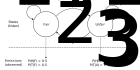
\includegraphics[width=8cm]{../../report/figure1}
			\caption{Простая скрытая марковская модель.} \label{fg:2}
		\end{figure}
		
		\note{	
			\begin{defenition}
				Путем $\pi$ называется последовательность состояний $\{z_i\}_{i=1}^{n}$ и наблюдаемых символов $\{y_i\}_{i=1}^{n}$ СММ.
				Последовательность $X$, которая была получена в результате прохода профильной СММ пути $\pi$, называется последовательностью наблюдаемых символов.
			\end{defenition}
											
			Примером простой СММ может быть модель, изображенная на слайде и описывающая подбрасывание двух монет. Пусть между наблюдателем и человеком с монетами стоит ширма, которая позволяет наблюдателю видеть только пол, куда падают монеты. Пусть есть две монеты: одна "--- честная монета, вторая "--- нечестная монета с перевесом в одну из сторон. Пусть человек с монетами с некоторой вероятностью либо подбрасывает монету, которую он бросил в прошлый раз, либо меняет монеты и бросает новую. При этом наблюдатель не знает, какая монета используется в конкретный момент времени, так как он не видит рук бросающего монеты и не может отличить одну монету от другой по их внешнему виду, он видит только последовательность результатов бросков.
		}
	\end{frame}

	\begin{frame}{Обозначения и известные результаты}				
		\begin{figure}[h]
			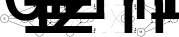
\includegraphics[width=11cm]{../../report/figure2}
			\caption{Профильная скрытая марковская модель.}  \label{fg:3}
		\end{figure}	
		
		Пусть даны $X$, $\overline{\omega} \in \overline{\Omega}$. Профильные СММ состоят из трех типов состояний, распределения которых строятся на основе $\overline{\omega}$ (Compeau Phillip, Pevzner Pavel 2015):
		\begin{itemize}
			\item S-состояние --- начальное состояние,
			\item М-состояния --- устанавливают соответствие символов в $X$ и $\overline{\omega}$,
			\item I-состояния и D-состояния --- устанавливает соответствие пропуска и символа в $X$ и $\overline{\omega}$,
			\item E-состояние --- конечное состояние.
		\end{itemize}
		
		\note{	
			Профильная СММ "--- это СММ со специальной линейной архитектурой состояний, которая позволяет выравнивать последовательность к множеству последовательностей.
			
			Пусть даны $X$, $\overline{\omega} \in \overline{\Omega}$.	Профильные СММ состоят из трех типов состояний, распределения которых строятся на основе $\overline{\omega}$:
			\begin{itemize}
				\item S-состояние --- начальное состояние,
				\item М-состояния --- устанавливают соответствие символов в $X$ и $\overline{\omega}$,
				\item I-состояния и D-состояния --- устанавливает соответствие пропуска и символа в $X$ и $\overline{\omega}$,
				\item E-состояние --- конечное состояние.
			\end{itemize}
		}
	\end{frame}

	\begin{frame}{Обозначения и известные результаты}				
		Алгоритмы профильных СММ позволяют по-разному оценивать выравнивание $X$ к $\overline{\omega}$ (Newberg Lee A. 2009; Rakesh Dugad 1996). 
		
		\begin{defenition}
			Вероятность пути $s(\pi)$ "--- произведение всех переходных вероятностей от состояний к состоянию и вероятностей наблюдаемых символов, которые излучаются в каждом состоянии, кроме начального и конечного, на протяжении всего пути $\pi$. 
		\end{defenition}		
		
		\begin{equation*}
			s_{max}(X) = \underset{\pi \in \pi_{X}}{max}(s(\pi)); \label{eq:1}
		\end{equation*}
		
		\begin{equation*}
			s_{fw}(X) = \sum_{\pi \in \pi_{X}}s(\pi), \label{eq:2}
		\end{equation*}
		
		где $\pi_{X}$ --- это путь, который мог излучить $X$.
		
		\note{	
			Алгоритмы профильных СММ позволяют по-разному оценивать выравнивание $X$ к $\overline{\omega}$. 
			
			\begin{defenition}
				Вероятность пути $s(\pi)$ "--- произведение всех переходных вероятностей от состояний к состоянию и вероятностей наблюдаемых символов, которые излучаются в каждом состоянии, кроме начального и конечного, на протяжении всего пути $\pi$. 
			\end{defenition}		
			
			\begin{equation*}
				s_{max}(X) = \underset{\pi \in \pi_{X}}{max}(s(\pi)); \label{eq:1}
			\end{equation*}
			
			\begin{equation*}
				s_{fw}(X) = \sum_{\pi \in \pi_{X}}s(\pi), \label{eq:2}
			\end{equation*}
			
			где $\pi_{X}$ --- это путь, который мог излучить $X$.
		}
	\end{frame}
	
	\setcounter{framenumber}{9}
	\begin{frame}{Обозначения и известные результаты}				
		Алгоритмы профильных СММ позволяют по-разному оценивать выравнивание $X$ к $\overline{\omega}$ (Newberg Lee A. 2009; Rakesh Dugad 1996).
		
		\begin{defenition}
			Вероятность пути $s(\pi)$ "--- произведение всех переходных вероятностей от состояний к состоянию и вероятностей наблюдаемых символов, которые излучаются в каждом состоянии, кроме начального и конечного, на протяжении всего пути $\pi$. 
		\end{defenition}		
		
		\begin{equation*}
			s_{max}(X) = \underset{\pi \in \pi_{X}}{max}(s(\pi)); \label{eq:1}
		\end{equation*}
		
		\begin{equation*}
			s_{fw}(X) = \sum_{\pi \in \pi_{X}}s(\pi), \label{eq:2}
		\end{equation*}
		
		где $\pi_{X}$ --- это путь, который мог излучить $X$.
		
		\note{	
			Вероятность Витерби $s_{max}(X)$ последовательности $X$ "--- это максимальная вероятность последовательности $X$ среди всех путей $\pi$, которые могли бы ее испустить:
			\begin{equation*}
				s_{max}(X) = \underset{\pi \in \pi_{X}}{max}(s(\pi)),
			\end{equation*}
			Несмотря на большое количество возможных путей, которые могли бы испустить последовательность $X$, алгоритм Витерби позволяет эффективно решать эту задачу.
			
			Форвард вероятность $s_{fw}(X)$ последовательности $X$ "--- это общая вероятность того, что в результате работы СММ будет получена последовательность $X$:
			\begin{equation*}
				s_{fw}(X) = \sum_{\pi \in \pi_{X}}s(\pi).
			\end{equation*}		
			Форвард алгоритм работает за то же время, что и алгоритм Витерби.
		}
	\end{frame}
		
	\begin{frame}{Обозначения и известные результаты}				
		\begin{equation*}
			Z(X, T)	= \sum_{\pi \in \pi_{X}}s(\pi)^{\frac{1}{T}}, \label{eq:3}
		\end{equation*}
		где $s(\pi)^{\frac{1}{T}}$ обозначает эквивалент вероятности $\pi$, который все еще вычисляется как произведение независимых событий, но каждый множитель возводиться в степень $\frac{1}{T}$.
		\note{	
			Третий способ оценивать последовательности, позволяющий уменьшить дисперсию дальнейших вычислений оценки ложноположительной вероятности оценки, заключается в том, что каждая вероятность перехода из одного состояния в другое и вероятность излучения символа состоянием будут возводится в степень $\frac{1}{T}$, где $T \in (0; +\infty)$. При этом логика вычислений остается та же, то есть $s(\pi)^{\frac{1}{T}}$ и $s(X)^{\frac{1}{T}}$ будут вычисляться как вероятность произведения независимых событий и как сумма непересекающихся событий соответственно, хотя они уже могут не являться вероятностями (Например, сумма всех $s(\pi)^\frac{1}{T}$ не обязательно равна единице):
			\begin{equation*}
				Z(X, T)	= \sum_{\pi \in \pi_{X}}s(\pi)^{\frac{1}{T}}.
			\end{equation*}		
			Функция $Z(X, T)$ называется статистической суммой и вычисляется через модификацию Форвард алгоритма. Параметра $T$ подбирается экспериментально под конкретную интересующую оценку выравнивания.
		}
	\end{frame}

	\begin{frame}{Обозначения и известные результаты}
		\begin{defenition}
			Моделью последовательностей называется генератор, моделирующий последовательности в соответствии с некоторым распределением. 
		\end{defenition}
	
		$P(X|M)$, где $M$ --- некоторая модель, означает условную вероятность $X$, при условии ее моделирования моделью $M$.
	
		\begin{defenition}
			Фоновой моделью $B$ для последовательностей длины $L$ называется генератор последовательностей длины $L$ такой, что все $L$ символьных позиций независимы и одинаково распределены:
			\begin{equation*}
				\mathsf{P}(X|B) = \prod_{i=1}^{L}\mathsf{P}(x_{i}|B), \label{eq:4}
			\end{equation*}
			где $x_i$ отражает возможный наблюдаемый символ.
		\end{defenition}
		
		\note{			
			\begin{defenition}
				Моделью последовательностей называется генератор, моделирующий последовательности в соответствии с некоторым распределением. 
			\end{defenition}
			
			$P(X|M)$, где $M$ --- некоторая модель, означает условную вероятность $X$, при условии ее моделирования моделью $M$.
			
			\begin{defenition}
				Фоновой моделью $B$ для последовательностей длины $L$ называется генератор последовательностей длины $L$ такой, что все $L$ символьных позиций независимы и одинаково распределены:
				\begin{equation*}
					\mathsf{P}(X|B) = \prod_{i=1}^{L}\mathsf{P}(x_{i}|B), \label{eq:4}
				\end{equation*}
				где $x_i$ отражает возможный наблюдаемый символ.
			\end{defenition}
		
			Фоновая модель описывает шум.
		}
		
	\end{frame}
	
	\begin{frame}{Обозначения и известные результаты}
		\begin{defenition}
			Ложноположительная вероятность оценки $s_{0}$ для строк длины $L$:	
			\begin{equation*}
				fpr(s_{0}) =  \sum_{X \in X_{L}} \mathsf{P}(X|B) \Theta(s(X) \geq s_{0}), \label{eq:5}
			\end{equation*}
			где $\mathsf{P}(X|B)$ "--- условная вероятность последовательности $X$, описываемая фоновой моделью, $s(X)$ "--- оценка последовательности $X$, считаемая профильной СММ, и
			\[
			\Theta(s(X) \geq s_{0}) = 
			\begin{cases}
				1, & s(X) \geq s_{0}\\
				0, & s(X) < s_{0}
			\end{cases}.
			\]
		\end{defenition}	
		
		\note{
			Последовательность $X$ длины $L$ сравнивается с остальными последовательностями той же длины. 
			\begin{equation*}
				fpr(s_{0}) =  \sum_{X \in X_{L}} \mathsf{P}(X|B) \Theta(s(X) \geq s_{0}),
			\end{equation*}
			где $\mathsf{P}(X|B)$ "--- условная вероятность последовательности $X$, описываемая фоновой моделью, $s(X)$ "--- оценка последовательности $X$, считаемая профильной СММ, и
			\[
			\Theta(s(X) \geq s_{0}) = 
			\begin{cases}
				1, & s(X) \geq s_{0}\\
				0, & s(X) < s_{0}
			\end{cases}.
			\]
			То есть $fpr(s_{0})$ "--- это вероятность того, что шум достигнет или превзойдет оценку $s_{0}$. В определении $fpr(s_{0})$ оценка $X$ отмечена как $s(X)$, потому что способ оценки последовательности может выбираться относительно интересующего приложения, подходит $s(X) = s_{max}(X)$ и $s(X) = s_{fw}(X)$.
		}
	\end{frame}
	
	\begin{frame}{Обозначения и известные результаты}
		Вычисление $fpr(s_{0})$ по определению обычно неосуществимо, значение $fpr(s_{0})$ может быть оценено через выборку по значимости. 
		
		\vspace{0.5cm}
		
		Пусть $\mathsf{P}(X|T)$ "--- это условная вероятность строки $X$ относительно некоторой модели строк длины $L$ параметризованной значением $T$. Тогда можно переписать $fpr(s_{0})$:		
		
		\begin{equation*}
			fpr(s_{0}) = \sum_{X \in X_{L}} \mathsf{P}(X|T) f(X,s_{0}), \label{eq:6}
		\end{equation*}
		где
		\begin{equation*}
			f(X,s_{0}) = \frac{\mathsf{P}(X|B) \Theta(s(X) \geq s_{0})}{\mathsf{P}(X|T)}. \label{eq:7}
		\end{equation*}		
		
		\note{
			Так как вычисление $fpr(s_{0})$ по определению обычно неосуществимо, значение $fpr(s_{0})$ может быть оценено через выборку по значимости, то есть через моделирование строк в соответствии с фоновой моделью $B$ и оценивание значения $fpr(s_{0})$ долей тех из них, что достигают оценки $s_{0}$.
			
			Построим распределение, относительно которого будем моделировать строки. Пусть $\mathsf{P}(X|T)$ "--- это условная вероятность строки $X$ относительно некоторой модели строк длины $L$ параметризованной значением $T$. Тогда можно переписать $fpr(s_{0})$:
			\begin{equation*}
				fpr(s_{0}) = \sum_{X \in X_{L}} \mathsf{P}(X|T) f(X,s_{0}),
			\end{equation*}
			где
			\begin{equation*}
				f(X,s_{0}) = \frac{\mathsf{P}(X|B) \Theta(s(X) \geq s_{0})}{\mathsf{P}(X|T)}.
			\end{equation*}
			Мы можем оценить значение $fpr(s_{0})$ через моделирование последовательностей в соответствии с этой альтернативной моделью и подсчет среднего значения $f(X,s_{0})$. Этот подход и называется выборкой по значимости, он полезен, потому что если правильно подобрать альтернативную модель, то удастся уменьшить дисперсию оценки $fpr(s_{0})$.
		}
	\end{frame}

	\begin{frame}{Обозначения и известные результаты}
		Определим распределение модели, используемой для выборки по важности параметризованную $T$:		
		
		\begin{equation*}
			\mathsf{P}(X|T) = \frac{\mathsf{P}(X|B)Z(X,T)}{Z(T)}, \label{eq:8}
		\end{equation*}							
		где 
		\begin{equation*}
			Z(T) = \sum_{X \in X_{L}}\mathsf{P}(X|B)Z(X,T). \label{eq:9}
		\end{equation*}
		Подставив определение $\mathsf{P}(X|T)$ в определение $f(X,s_{0})$, получим
		\begin{equation*}
			f(X,s_{0}) = \frac{Z(T)\Theta(s(X) \geq s_{0})}{Z(X|T)}. \label{eq:10}
		\end{equation*}	
		
		\note{
			Определим распределение модели, используемой для выборки по важности параметризованную $T$ следующим образом:
			\begin{equation*}
				\mathsf{P}(X|T) = \frac{\mathsf{P}(X|B)Z(X,T)}{Z(T)},
			\end{equation*}							
			где 
			\begin{equation*}
				Z(T) = \sum_{X \in X_{L}}\mathsf{P}(X|B)Z(X,T).
			\end{equation*}	
			Подставив определение $\mathsf{P}(X|T)$ в определение $f(X,s_{0})$, получим 
			\begin{equation*}
				f(X,s_{0}) = \frac{Z(T)\Theta(s(X) \geq s_{0})}{Z(X|T)}.
			\end{equation*}							
		}
	\end{frame}
	
	\begin{frame}{Обозначения и известные результаты}
			Моделируем $\{X_i\}_{i=1}^N$ в соответствии с распределением $\mathsf{P}(X|T)$ (Newberg Lee A. 2009), вычисляем $f(X, s_{0})$ для каждой последовательности и использовать среднее этих значений как оценку $fpr(s_{0})$:
			
			\begin{equation*}	
				\widehat{fpr}(s_{0}) = \frac{Z(T)}{N} \sum_{1}^{N} \frac{\Theta(s(X_{i}) \geq s_{0})}{Z(X_{i}, T)}
			\end{equation*}	
		
		\note{
			Моделируем $\{X_i\}_{i=1}^N$ в соответствии с распределением $\mathsf{P}(X|T)$, вычисляем $f(X, s_{0})$ для каждой последовательности и использовать среднее этих значений как оценку $fpr(s_{0})$:
			
			\begin{equation*}	
				\widehat{fpr}(s_{0}) = \frac{Z(T)}{N} \sum_{1}^{N} \frac{\Theta(s(X_{i}) \geq s_{0})}{Z(X_{i}, T)}
			\end{equation*}	
			
			Опуская подробности того как устроены моделирование, построенное на модификациях классических алгоритмов, связанных с HMM, и метод подбора параметра $T$, перейдем к полученным результатам.
		}
	\end{frame}
		
	\begin{frame}{Полученные результаты}
		Вычислим оценку $\widehat{fpr}(s_{0})$ для строк длины $L=100$, состоящих из 5 символов, и доверительные интервалы уровня $\gamma = 0.99$:		
		\begin{table}
			\caption{Результаты.} \label{tb:1}
			\begin{tabular}{cccc}
				$s_{0}$&T&$\widehat{fpr}(s_{0})$&$[c_{1}(\gamma);c_{2}(\gamma)]$  \\ \hline
				$10^{-85}$&7&0.0000000183&[0.0; 0.00066349] \\
				$10^{-90}$&7&0.003175&[0.001884; 0.004779] \\ 
				$10^{-100}$&7&0.615709&[0.597540 0.622677] \\
			\end{tabular}
		\end{table}	
		
		\note{
			Вычислим оценку $\widehat{fpr}(s_{0})$ для строк длины $L=100$ и доверительные интервалы уровня $\gamma = 0.99$:
			\begin{center}
				\begin{tabular}{cccc}
					$s_{0}$&T&$\widehat{fpr}(s_{0})$&$[c_{1}(\gamma);c_{2}(\gamma)]$  \\ \hline
					$10^{-85}$&7&0.0000000183&[0.0; 0.00066349] \\
					$10^{-90}$&7&0.003175&[0.001884; 0.004779] \\ 
					$10^{-100}$&7&0.615709&[0.597540 0.622677] \\
				\end{tabular}
			\end{center}
			Вычисление $fpr(s_{0})$ перебором привело бы к перебору $5^{100}$ строк.
		}
	\end{frame}
	
	\begin{frame}{Заключение}
		\begin{itemize}
			\item Была изучена тема алгоритмов парного и множественного выравнивания последовательностей и тема СММ и алгоритмов взаимодействия с ними.
			\item Был реализован алгоритм, позволяющий эффективно вычислять оценку ${fpr}(s_{0})$.
			\item Предстоит подробно верифицировать реализованный алгоритм и сравнить его с имеющимися методами вычисления оценки ${fpr}(s_{0})$.
		\end{itemize}
		
		\note{
			\begin{itemize}
				\item Была изучена тема алгоритмов парного и множественного выравнивания последовательностей и тема СММ и алгоритмов взаимодействия с ними.
				\item Был реализован алгоритм, позволяющий эффективно вычислять оценку ${fpr}(s_{0})$.
				\item Предстоит подробно верифицировать реализованный алгоритм и сравнить его с имеющимися методами вычисления оценки ${fpr}(s_{0})$.
			\end{itemize}
		}
	\end{frame}	
	
\end{document}
